\renewcommand{\theequation}{\theenumi}
\begin{enumerate}[label=\thesection.\arabic*.,ref=\thesection.\theenumi]
\numberwithin{equation}{enumi}

\item A conic section has the following equation\ref{eq:alg_conic}
\begin{align}
Ax^2+Bxy+Cy^2+Dx+Ey+F=0
\label{eq:alg_conic}
\end{align}
The equation is expressed in vector form is as follows
The vector form is 
\begin{align}
\label{eq:vec_conic}
\vec{x}^T \myvec{A & B/2\\B/2 & C}\vec{x}+ \myvec{D & E}\vec{x}+F=0
\end{align}
If $x_1$ is root of an equation ,Then $\brak{x-x_1}$ is a factor
\item 
\begin{align}
\label{eq:alg_conic_a}
\brak{a} 12x^{2} - 7x + 1
\end{align}
can be expressed according to \ref{eq:vec_conic} as 
\begin{align}
\label{eq:vec_conic_a}
\vec{x}^T \myvec{12 & 0\\0 & 0}\vec{x}+ \myvec{-7 & 0}\vec{x}+1=0
\end{align}
To find roots using \ref{eq:vec_conic_a}, substitute
\begin{align}
y=0
\\
\implies 
12x^{2}-7x+1=0
\\
x=\frac{1}{3}, \frac{1}{4}
\end{align}
Hence $\brak{x-\frac{1}{3}}$ and $\brak{x-\frac{1}{4}}$ are the factors
\begin{align}
\implies \brak{3x-1}\brak{4x-1}=12x^{2} - 7x + 1 
\end{align}

The following code sketches the graph of \ref{eq:alg_conic_a} in figure \ref{fig:conic2a}
\begin{lstlisting}
codes/conic2/conic2a.py
\end{lstlisting}
\begin{figure}[!ht]
\centering
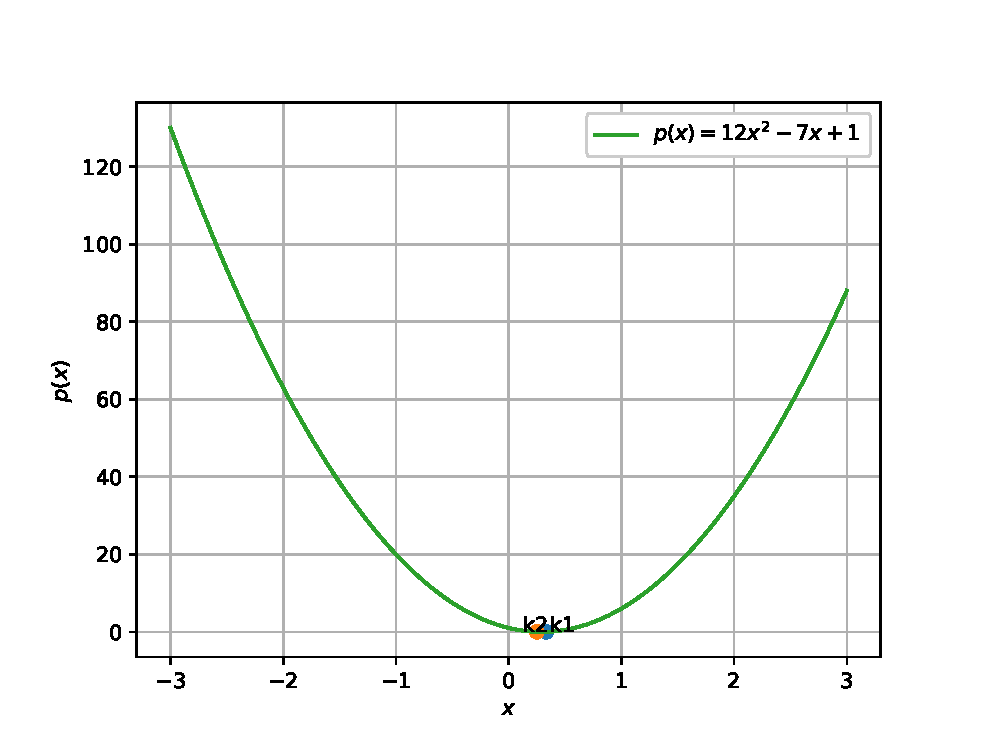
\includegraphics[width=\columnwidth]{./codes/conic2/pyfigs/conic2a.eps}
\caption{Graph of $12x^{2} - 7x + 1$}
\label{fig:conic2a}
\end{figure}


\item 
\begin{align}
\label{eq:alg_conic_b}
\brak{b} 6x^{2} + 5x -6
\end{align}
can be expressed according to \ref{eq:vec_conic} as 
\begin{align}
\label{eq:vec_conic_b}
\vec{x}^T \myvec{6 & 0\\0 & 0}\vec{x}+ \myvec{5 & 0}\vec{x} -6 =0
\end{align}
Substituting $y=0$ in equation \ref{eq:vec_conic_b} to find roots,
\begin{align}
\implies 
6x^{2}+5x-6=0
\\
x=\frac{-3}{2}, \frac{2}{3}
\\
\brak{2x+3}\brak{3x-2}= 6x^{2} + 5x -6
\end{align}
The following code sketches the graph of \ref{eq:alg_conic_b} in figure \ref{fig:conic2b}
\begin{lstlisting}
codes/conic2/conic2b.py
\end{lstlisting}
\begin{figure}[!ht]
\centering
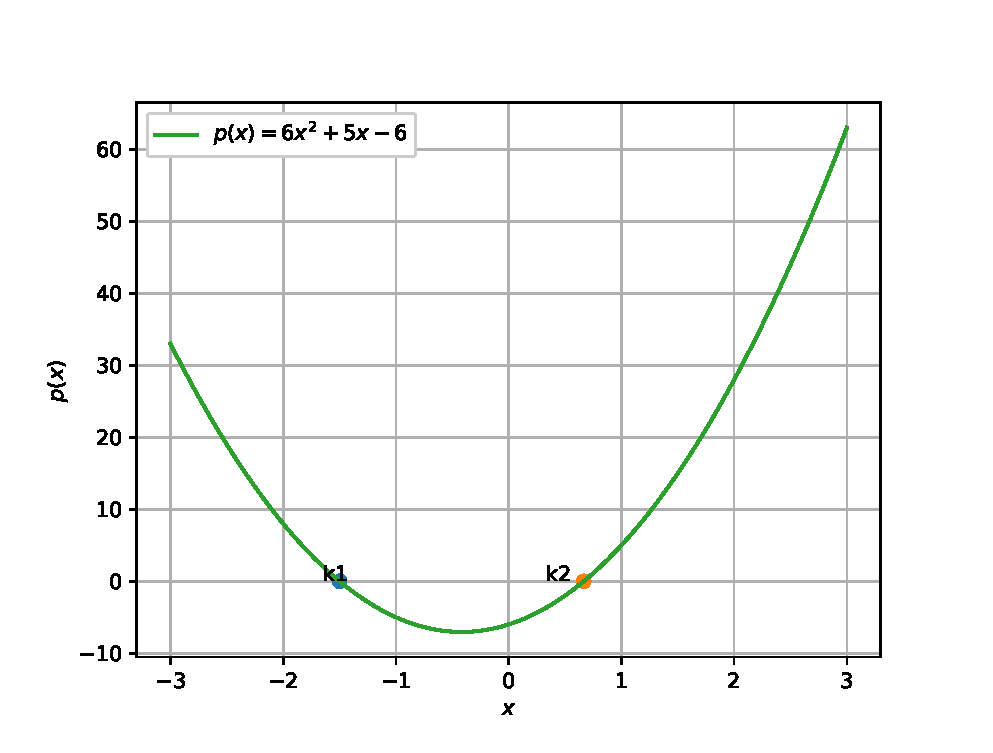
\includegraphics[width=\columnwidth]{./codes/conic2/pyfigs/conic2b.eps}
\caption{Graph of $6x^{2} + 5x -6$}
\label{fig:conic2b}
\end{figure}

\item 
\begin{align}
\label{eq:alg_conic_c}
\brak{c} 2x^{2} + 7x +3
\end{align}
can be expressed according to \ref{eq:vec_conic} as 
\begin{align}
\label{eq:vec_conic_c}
\vec{x}^T \myvec{2 & 0\\0 & 0}\vec{x}+ \myvec{7 & 0}\vec{x} +3 =0
\end{align}
Substituting $y=0$ in equation \ref{eq:vec_conic_c},
\begin{align}
\implies 
2x^{2}+7x+3=0
\\
x=\frac{-1}{2},-3
\\
\brak{2x+1}\brak{x+3}= 2x^{2} + 7x +3
\end{align}

The following code sketches the graph of \ref{eq:alg_conic_c} in figure \ref{fig:conic2c}
\begin{lstlisting}
codes/conic2/conic2c.py
\end{lstlisting}
\begin{figure}[!ht]
\centering
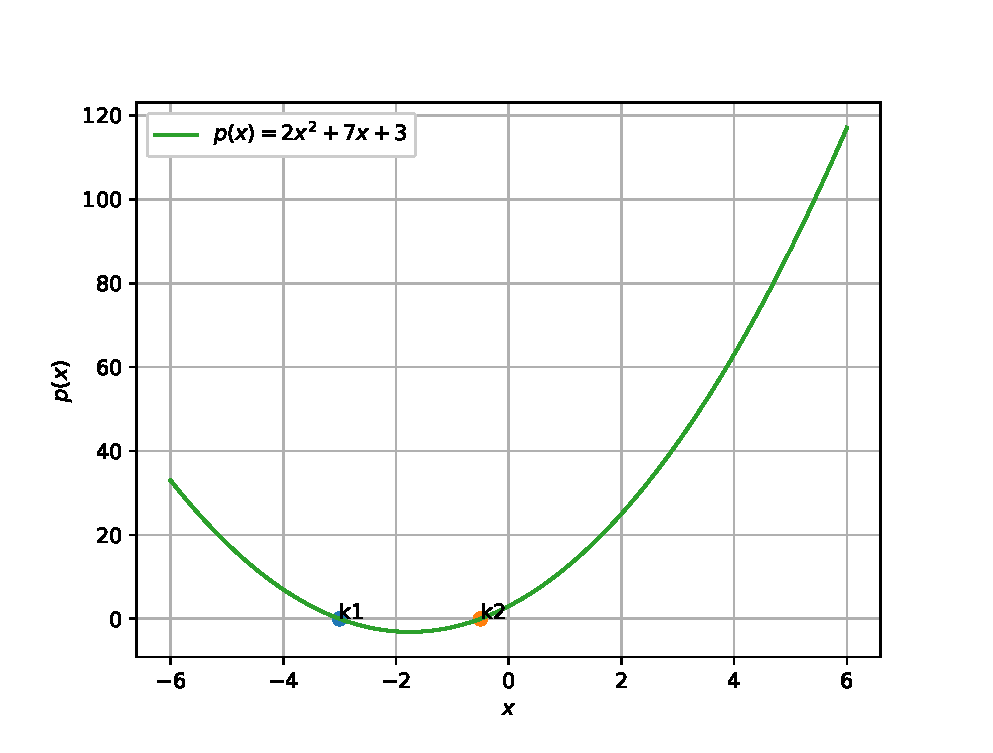
\includegraphics[width=\columnwidth]{./codes/conic2/pyfigs/conic2c.eps}
\caption{Graph of $2x^{2} + 7x +3$}
\label{fig:conic2c}
\end{figure}


\item 
\begin{align}
\label{eq:alg_conic_d}
\brak{d} 3x^{2} -x -4
\end{align}
can be expressed according to \ref{eq:vec_conic} as 
\begin{align}
\label{eq:vec_conic_d}
\vec{x}^T \myvec{3 & 0\\0 & 0}\vec{x}+ \myvec{-1 & 0}\vec{x} -4 =0
\end{align}
Substituting $y=0$ in equation \ref{eq:vec_conic_c},
\begin{align}
\implies 
3x^{2}-x-4=0
\\
x=\frac{4}{3},-1
\\
\brak{3x-4}\brak{x+1}= 3x^{2} -x -4
\end{align}

The following code sketches the graph of \ref{eq:alg_conic_d} in figure \ref{fig:conic2d}
\begin{lstlisting}
codes/conic2/conic2d.py
\end{lstlisting}
\begin{figure}[!ht]
\centering
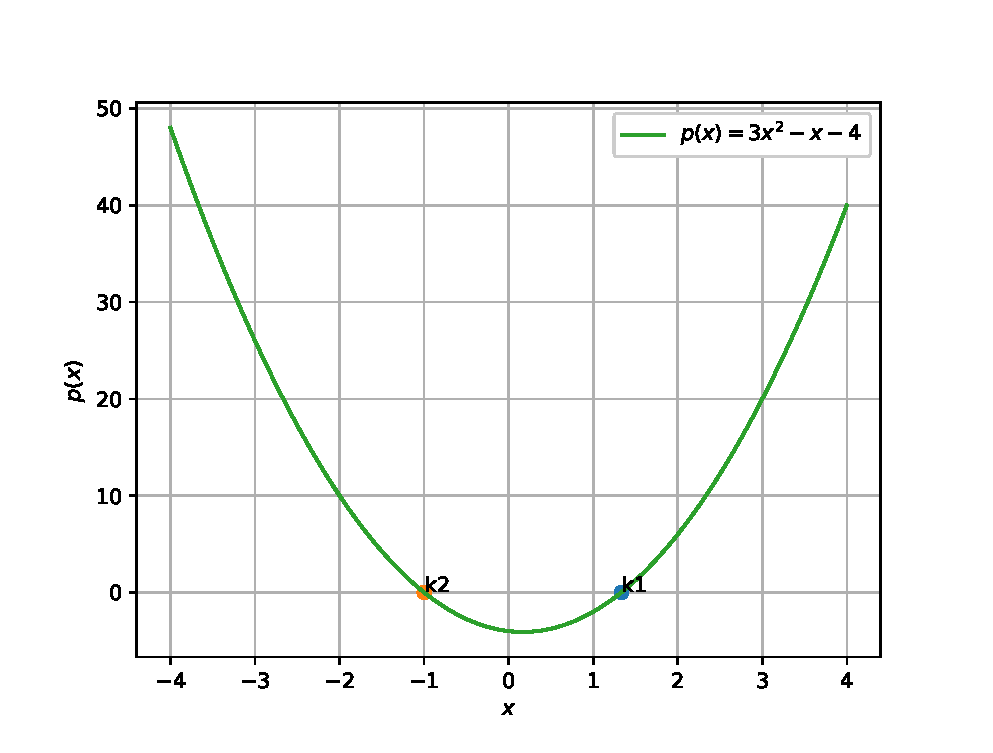
\includegraphics[width=\columnwidth]{./codes/conic2/pyfigs/conic2d.eps}
\caption{Graph of $3x^{2} -x -4$}
\label{fig:conic2d}
\end{figure}


\end{enumerate}
